\section{Experimental set-up}
The set-up consists in :
\begin{itemize}
\item A camera that films the movements of a servo configuration.
\item A simulation of that servo configuration in V-Rep.
\end{itemize}

\begin{figure}[htp]
\center
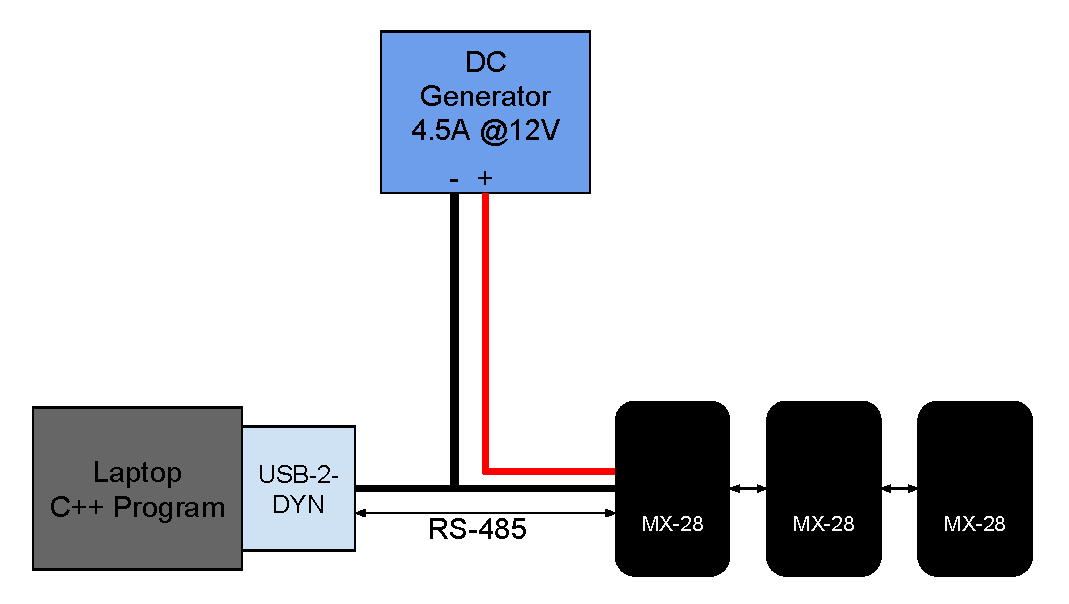
\includegraphics[width=0.6\textwidth]{figures/exp_setup}
\caption{Experimental setup}
\label{fig:exp_setup}
\end{figure}

\section{Experiments}
The first experiment is to test the torque : to that end, a frame is fixed onto a single servo and weighted. The setup is represented on \cref{fig:exp1}.

At $12V$, the maximal torque\cite{mx_28_manual} of the servo is supposedly $2.5N.m$. To test this, a weight of $2kg$ is hanged at $12.5cm$ from the center of the servo, because since 
\begin{align*}
2.5 - 9.81 \cdot (0.007 \cdot 0.01 + 0.016 \cdot 0.0725) &= x \cdot 0.125\\
x &= 20 N\\
&= 2.03 kg
\end{align*}

\begin{figure}[htp]
\center
    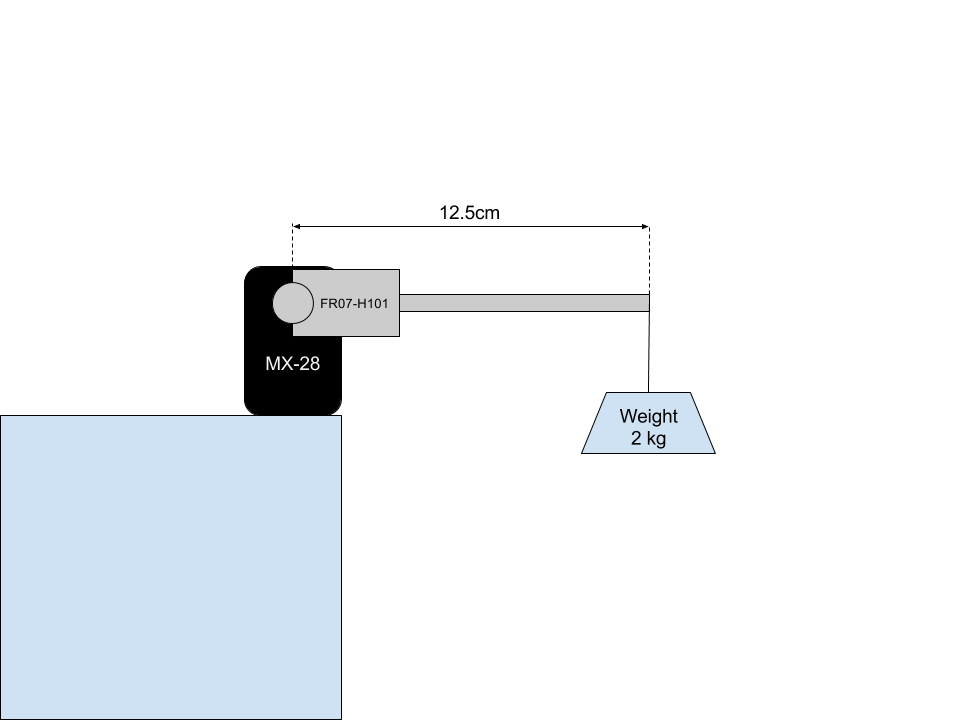
\includegraphics[width = 0.5\textwidth]{figures/exp1}
    \caption[Experimental setup for torque testing]{Experimental setup for torque testing : A weight of $2kg$ is suspended at $12.5cm$ from the servo, resulting in a torque of $2.5Nm$. The goal is to test whether the servo is able to move the weight upwards from the depicted initial situation.}
    \label{fig:exp1}
\end{figure}

Results
\begin{table}[htp]
\center
\begin{tabularx}{\textwidth}{@{}l X X X @{}}
\toprule
& \textbf{Stall torque @11.1V $[N.m]$} & \textbf{Stall torque @12V $[N.m]$} & \textbf{Stall torque @14.8V $[N.m]$}\\ 
\midrule
\textbf{Theoretical} & 2.1 & 2.5 & 3.1\\ 
\textbf{Experimental} &  &  & \\ 
\bottomrule
\end{tabularx}
\caption{Experimental stall torques at different tested voltages}
\label{table:exp1_results}
\end{table}

\section{Servo tuning}

\section{Results}